\documentclass[12pt,twoside,openright]{report} 


\usepackage{examplepackage}
\title{Research Paper}
\author{Himanshu Sharma}
\date{\today}


\setlength{\marginparwidth}{0pt}
\setlength{\oddsidemargin}{20pt}
\setlength{\textwidth}{450pt}


\setlength{\topmargin}{0.0in}
\setlength{\oddsidemargin}{0.33in}
\setlength{\evensidemargin}{-0.08in}
\setlength{\textheight}{8.5in}
\setlength{\textwidth}{6.0in}


\begin{document}
%\layout

\maketitle
\pagebreak

\section{Introduction}
\subfile{sections/Introduction}


\subfile{sections/mathematical_model}

% \section{Numerical Method and Software}

% \section{Results and Discussion}

% \subsection{Lithiation}
% \subsubsection{Effect of Young's modulus of SEI on Delamination during Lithiation}
% \begin{figure}[H]
%     \centering
%     \includegraphics[width=\textwidth]{plots/Lithiation/VariationWithE_SEI_bestFit.eps}
%     \caption{Variation of crack length with increasing Young's modulus of SEI ($E_{\textrm{SEI}}$) for the same level of charging (SOC=3\%)}
%     \label{fig:plot1}
% \end{figure}


% It was observed in the simulations that during lithiation, the SEI delaminates from the Si thin film. To investigate the effect of Young's modulus of SEI on the extent of delamination, a parametric study is carried out. To quantify the extent of delamination, the length to which the crack propagates has been chosen and has been non-dimensionalized. let $\delta(X)$ denote the gap between the two films, where $X$ denotes the material coordinates. Then $\overline{\delta}(X) = \frac{\delta}{L}$ is the non-dimensional gap distance. For quantifying the crack length, the non dimensional material coordinate($\overline{X} = \frac{X}{L}$) at which $\overline{\delta} = 10^{-5}$ has been taken. Fig \ref{fig:plot1} shows the effect of $E_{\textrm{SEI}}$ on the length of crack for different values of $G$ . It was observed that on increasing the young's modulus of the SEI, the crack length increases. This indicates that as the SEI gets stiffer it delaminates more easily from the Si film. From fig \ref{fig:plot1}
% it can also be observed that for a higher value of $G$, the crack length is less.

% \pagebreak

% \subsubsection{Effect of Interfacial bonding energy of SEI-Si interface on Delamination during Lithiation}
% \begin{figure}[h]
%     \centering
%     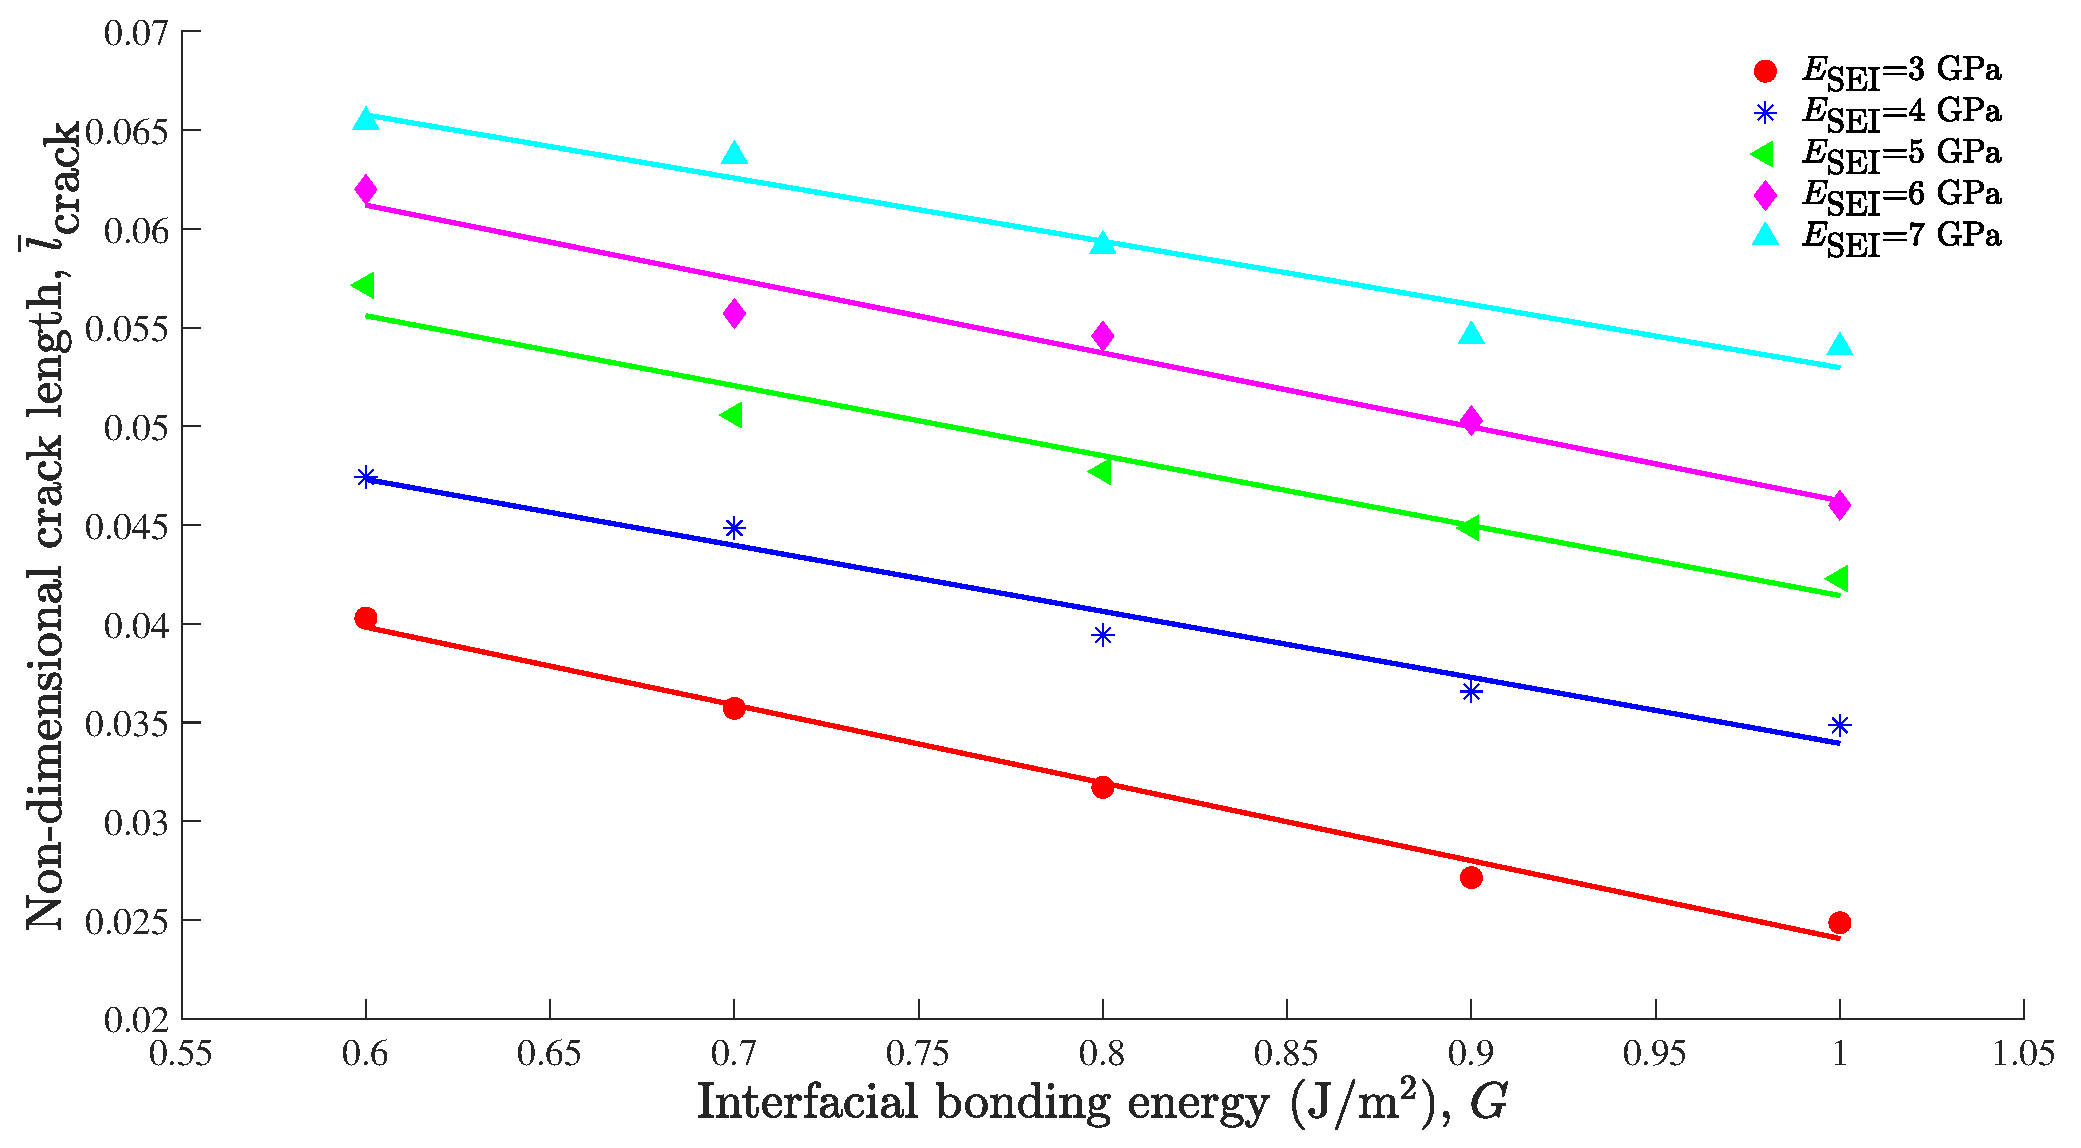
\includegraphics[width=\textwidth]{plots/Lithiation/VariationWithA_BestFit.eps}
%     \caption{Variation of crack length with increasing interfacial bonding energy (G) for the same level of charging (SOC=3\%)}
%     \label{fig:plot2}
% \end{figure}
% Interfacial bonding energy ($G$) of the SEI-Si interface plays an important role in the design of an artificial SEI layer. Fig \ref{fig:plot2} shows how the interfacial bonding energy affects the delamination for different value of $E_{\textrm{SEI}}$. It was observed that increasing $G$ lowers the extent of delamination. This happens because increasing the bonding energy of the interface leads to better strength of the interface. Moreover, it can be observed that for a higher Young's modulus of SEI the crack length is more. \\


% \pagebreak


% \subsubsection{Combined effect of $G$ and $E_{\textrm{SEI}}$ on Delamination during Lithiation}

% \begin{figure}[H]
%     \centering
%     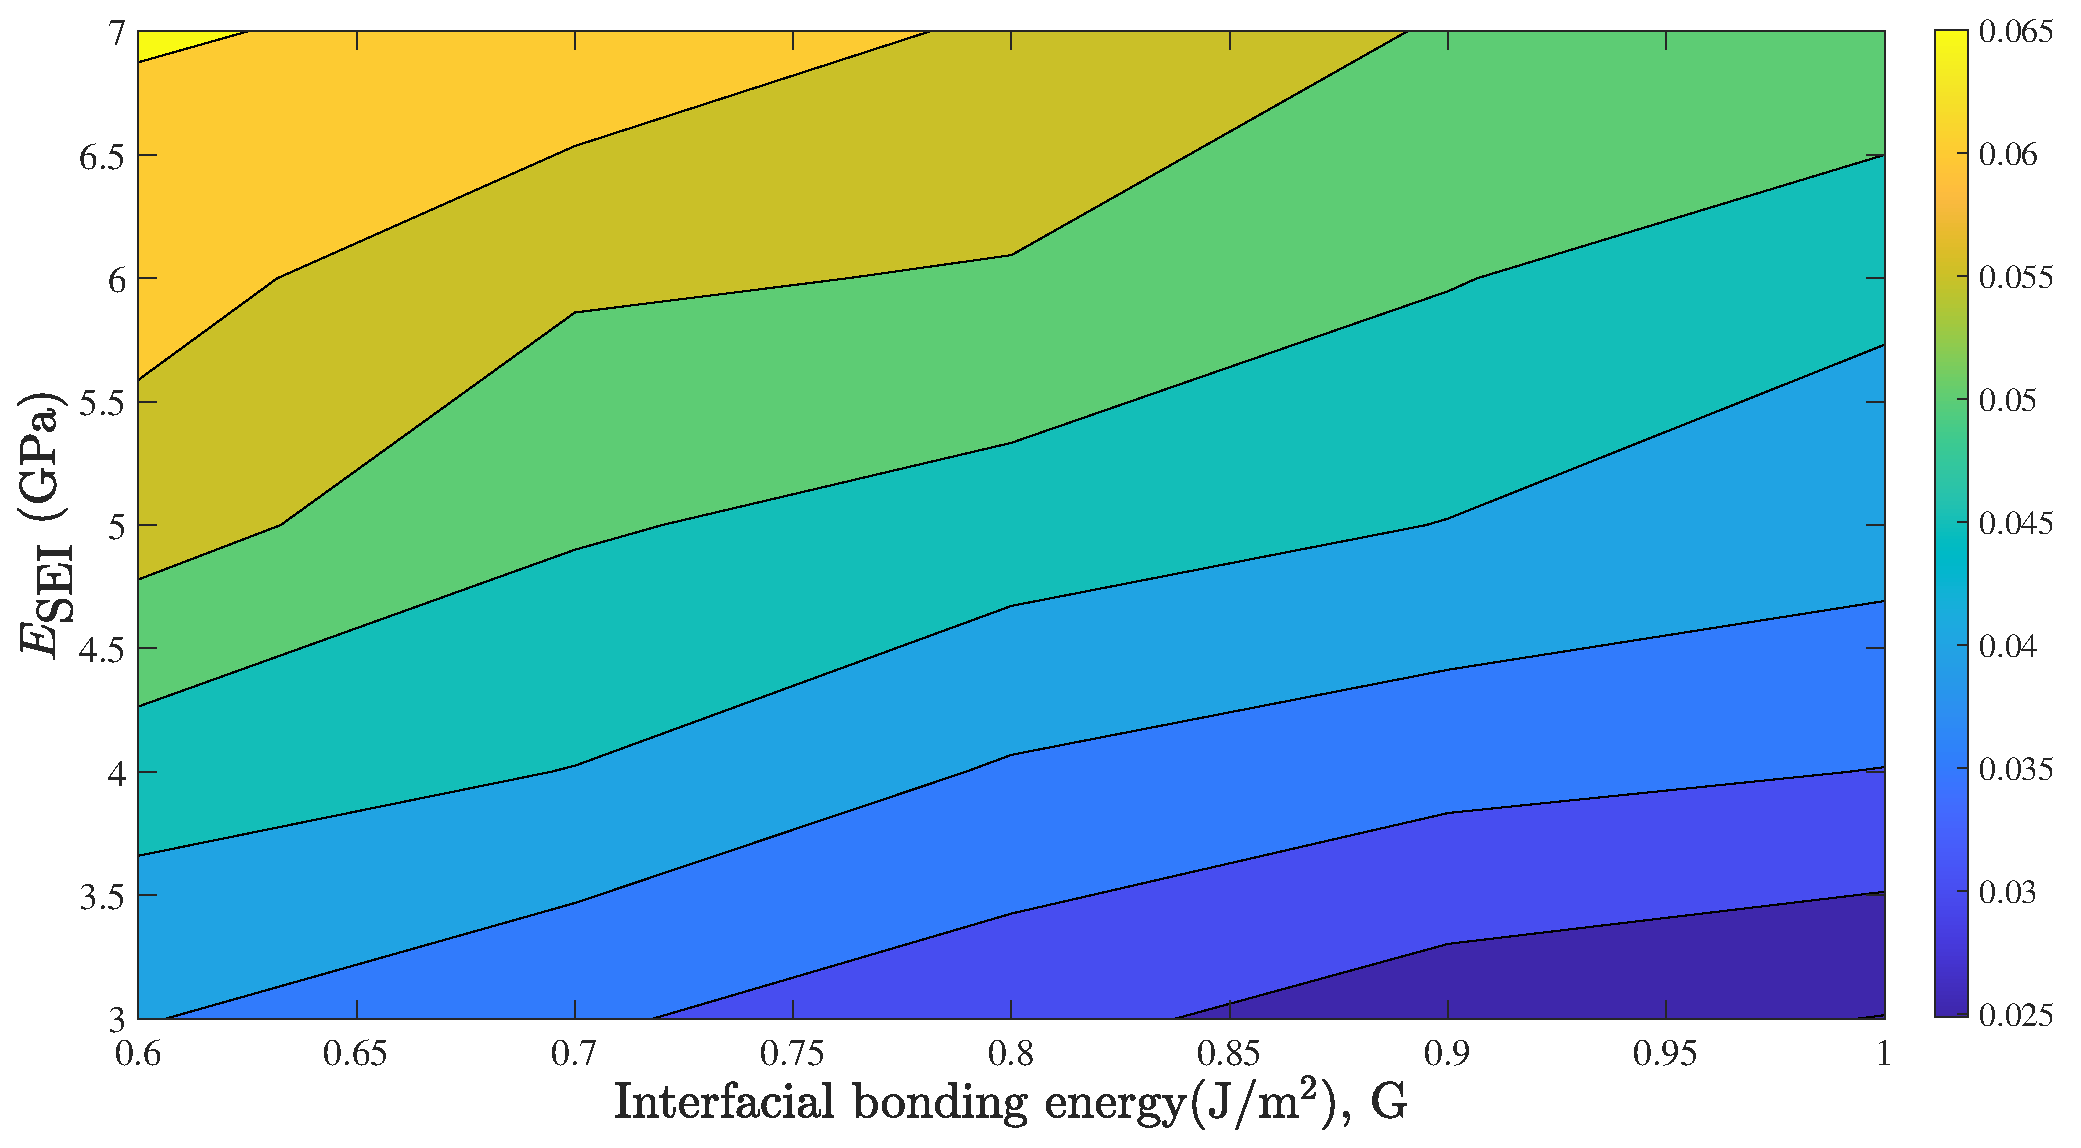
\includegraphics[width=\textwidth]{plots/Lithiation/ContourPlot.eps}
%     \caption{Variation of $\overline{l}_{\textrm{crack}}$ with $G$ and $E_{\textrm{SEI}}$}
%     \label{fig:plot3}
% \end{figure}

% Based on the above two parametric study, to design an SEI layer with good mechanical stability it should have low elastic modulus ($E_{\textrm{SEI}}$) and the corresponding interface should have high bonding energy ($G$). And as evident from fig \ref{fig:plot3} low Young's modulus of SEI and high interfacial bonding energy ensures that the length of crack is less. \\
% It can be observed from the best fit lines in figure \ref{fig:plot1} and \ref{fig:plot2} that $\overline{l}_{\textrm{crack}}$ varies approximately linearly with both $E_{\textrm{SEI}}$ and $G$. Based on the numerical results obtained $\overline{l}_{\textrm{crack}}$ can be approximated as
% \begin{equation}
% \overline{l}_{\textrm{crack}} = \textrm{0.0067943}E_{\textrm{SEI}}  -\textrm{0.035543}G + \textrm{0.041297}
% \end{equation}
% where $E_{\textrm{SEI}}$ is in GPa and $G$ is in J/m$^2$

% \pagebreak

% \subsubsection{Effect of Interface stiffness on Delamination during Lithiation}
% \pagebreak
% \subsubsection{Effect of Heterogeneity on Delamination during Lithiation}
% \pagebreak




% \subsection{Delithiation}
% \subsubsection{Effect of Young's modulus of SEI on Delamination during Delithiation}
% \pagebreak
% \subsubsection{Effect of Interfacial bonding energy of SEI-Si interface on Delamination during Delithiation}
% \pagebreak
% \subsubsection{Combined effect of $G$ and $E_{\textrm{SEI}}$ on Delamination during Delithiation}
% \pagebreak
% \subsubsection{Effect of Interface stiffness on Delamination during Delithiation}
% \pagebreak
% \subsubsection{Effect of Heterogeneity on Delamination during Delithiation}
% \pagebreak


% \begin{figure}[H]
%     \centering
%     \includegraphics[width=\textwidth]{sigmar - GFPDE.png}
%     \caption{$\CS_\textrm{r}$ in GFPDE module}
% \end{figure}

% \begin{figure}[H]
%     \centering
%     \includegraphics[width=\textwidth]{sigmar - SM.png}
%     \caption{$\CS_\textrm{r}$ in SM module}
% \end{figure}

% \begin{figure}[H]
%     \centering
%     \includegraphics[width=\textwidth]{u - GFPDE.png}
%     \caption{$\u$ in GFPDE module}
% \end{figure}

% \begin{figure}[H]
%     \centering
%     \includegraphics[width=\textwidth]{u - SM.png}
%     \caption{$u$ in SM module}
% \end{figure}

% \begin{figure}[H]
%     \centering
%     \includegraphics[width=\textwidth]{diff - tau_r.png}
%     \caption{difference between the internally defined $\bm{\tau}_{\text{r}}$ and self defined $\bm{\tau}_{\text{r}}$ in SM module}
% \end{figure}



\end{document}
